% ==================== 2.4.4 镜面 ====================
\subsubsection{镜面（\texorpdfstring{$P\,m\,\bar3$}{Pm-3}）}

镜面 $m$ 是一个对称平面，其操作前后两原子位于镜面同一法向的两侧、等距反向。为观察
镜面操作，选用空间群 $P\,m\,\bar3$（No.~200，立方晶系）：其点群 $m\,\bar3$ 由 3 组
互相垂直的镜面、4 个沿体对角线的 3 次轴、3 个 2 次轴及反演中心组合而成，其中镜面
垂直于三个晶轴方向，便于观察原子的镜像成对关系。建模参数见表~\ref{tab:sym-mir}。

\begin{table}[H]
  \centering
  \caption{镜面演示的建模参数}
  \label{tab:sym-mir}
  \begin{tabular}{ll}
    \toprule
    项目 & 参数 \\
    \midrule
    空间群 & $P\,m\,\bar3$（No.~200，立方晶系） \\
    晶格常数 & $a=b=c=5.0$\,\AA，$\alpha=\beta=\gamma=90^\circ$ \\
    原子坐标 & Si：$(0.2,\,0.3,\,0.4)$（一般位置） \\
    等效位置数 & 24（单胞内 24 个原子） \\
    \bottomrule
  \end{tabular}
\end{table}

\begin{figure}[H]
  \centering
  \subcaptionbox{(a) 空间群与晶胞参数设置}{%
    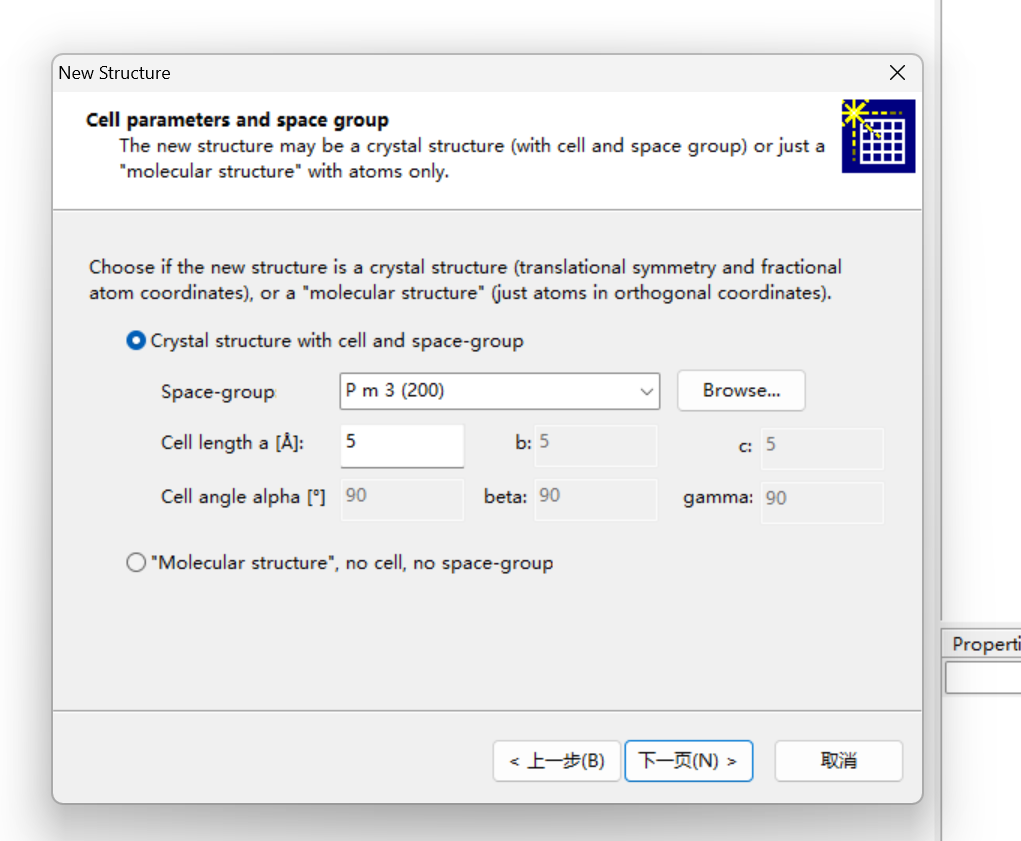
\includegraphics[width=0.44\textwidth]{assets/symmetry/mirror/a.png}}
  \hfill
  \subcaptionbox{(b) 非对称单元原子（Si）添加}{%
    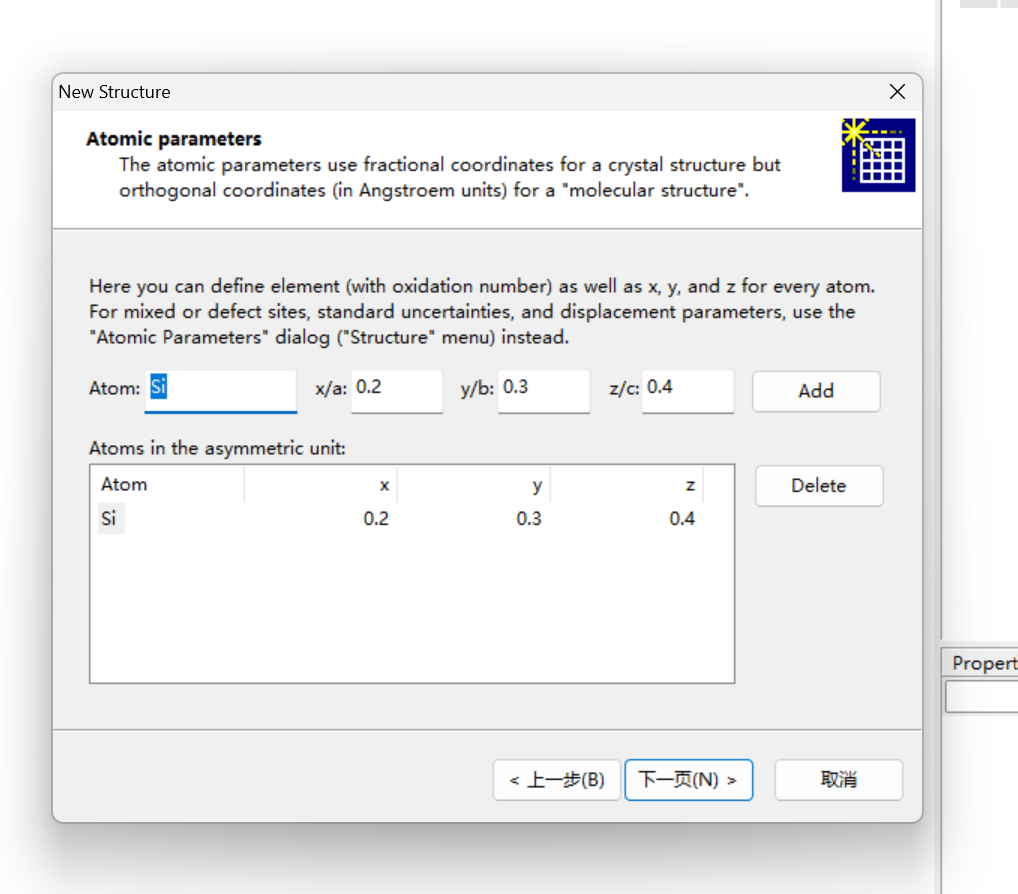
\includegraphics[width=0.44\textwidth]{assets/symmetry/mirror/b.png}}
  \caption{镜面（$P\,m\,\bar3$）演示的参数设置}
  \label{fig:sym-mir-param}
\end{figure}

\begin{figure}[H]
  \centering
  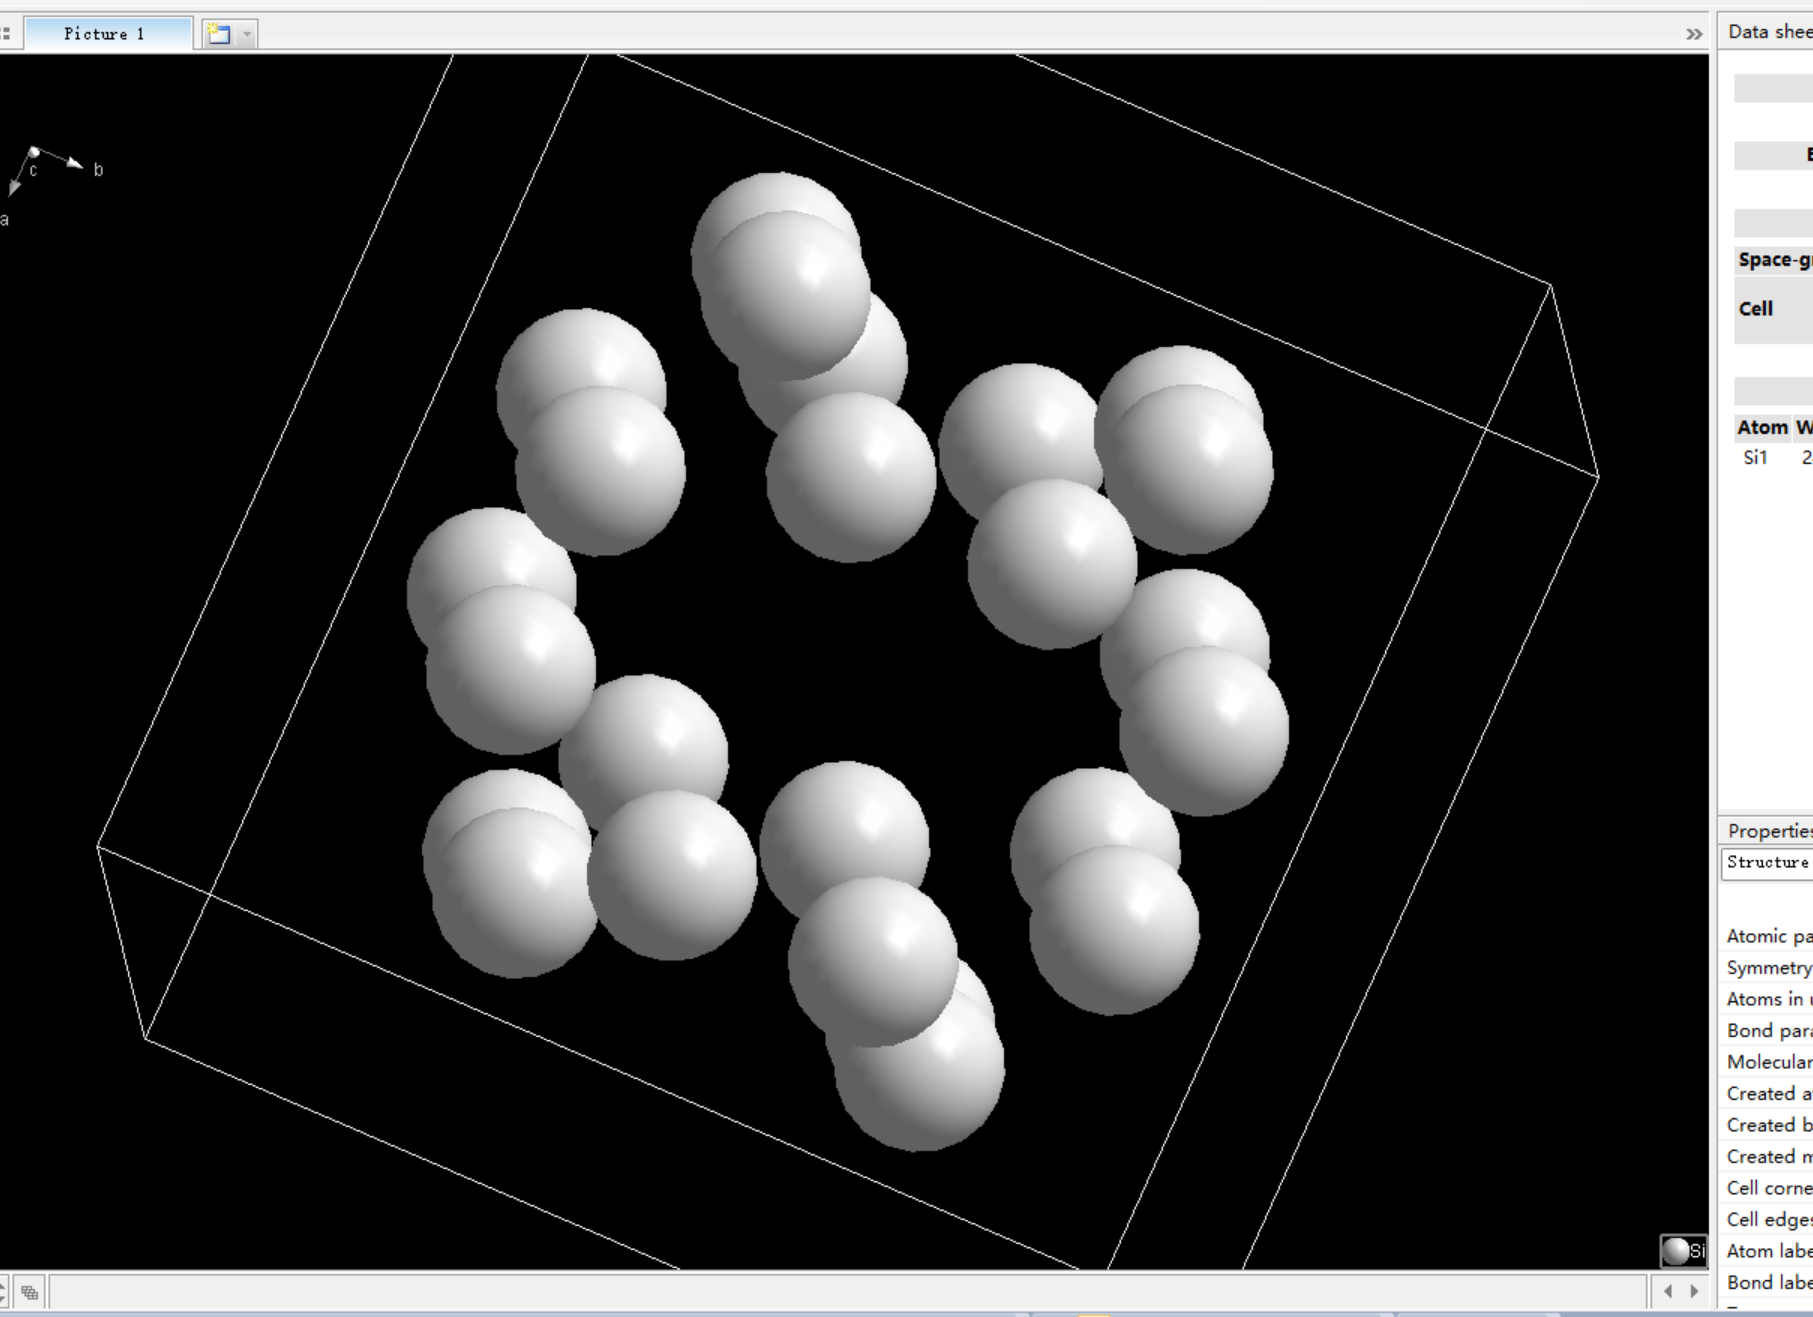
\includegraphics[width=0.5\textwidth]{assets/symmetry/mirror/c.png}
  \caption{镜面（$P\,m\,\bar3$）的单胞模型：24 个等效原子关于三组互相垂直的镜面
    镜像分布}
  \label{fig:sym-mir-model}
\end{figure}

$P\,m\,\bar3$ 中垂直于三个晶轴的镜面操作可分别写为
\begin{equation}
  \begin{aligned}
    m_{\perp a}:\ (x,y,z)\to(\bar x,\,y,\,z),&\qquad
    m_{\perp b}:\ (x,y,z)\to(x,\,\bar y,\,z),\\
    m_{\perp c}:\ (x,y,z)\to(x,\,y,\,\bar z).&
  \end{aligned}
\end{equation}
以 Si 的坐标 $(0.2,0.3,0.4)$ 为例，其关于三个镜面的像分别为 $(0.8,0.3,0.4)$、
$(0.2,0.7,0.4)$ 与 $(0.2,0.3,0.6)$。这些镜面操作与 4 个 3 次轴（体对角线方向）、
3 个 2 次轴、反演中心相互组合，在单胞内共生成 24 个等效原子
（图~\ref{fig:sym-mir-model}）。由于 24 个原子在晶胞内间距较小，图中原子显得较为
密集；实际观察时可旋转模型并利用 Atom Design 适当减小原子显示半径，即可清晰看到
原子关于镜面的成对镜像关系。

\textbf{特征与辨识要点。}镜面操作的显著特征是原子``镜像成对''：每组原子对位于镜面
两侧、与镜面等距且连线垂直于镜面。镜面不含任何平移分量，属宏观对称元素，镜面操作
还可以等效地记为 $\bar2$（二次旋转反演轴）。在 $P\,m\,\bar3$ 中，三组镜面互相垂直，
分别垂直于 $a$、$b$、$c$ 轴；镜面与 3 次轴、2 次轴及反演中心的组合使一般位置的多
重度达到 24。与镜面外形相似但含平移分量的对称元素是滑移面（见 2.4.6 节），两者的
区别只有在观察超晶胞时才能直接看出。
